%!TEX root = ../main.tex

%%%%%%%%%%%%%%%%%%%%%%%%%%%%%%%
%%%%%%%%%%%%%%%%%%%%%%%%%%%%%%%
\chapter{Methodical Modeling}
\label{chap:methodical-modeling}

\begin{textblock*}{.7\textwidth}(70mm-\offset,25mm-\offset)
        \begin{fquote}[Albert Einstein]
            All models are wrong, but some are useful.
        \end{fquote}
\end{textblock*}

This chapter mehodical modeling focusses on the description of thoughs and structures of the implementation in Python.
It is not evolving more than necessary details about the package {\itshape diffpssi}, but trying to comprehensible illustrate the structure of the algorithms theirselves and the necessaary bordering interfaces.

%%%%%%%%%%%%%%%%%%%%%%%%%%%%%%%
%%%%%%%%%%%%%%%%%%%%%%%%%%%%%%%
\section{Transformer Equipment Modeling}
\label{sec:transformer-modeling}

This section respectively focusses on the dynamics and model behavior of the transformer itself.
It is split according to the structure of the implementation itself, into the modeling of the $\Pi$-model and the tap changer control.
For the last mentioned, there are different control schemes implemented and thus described in the subsequent section.
In the beginning, the rough software structure idea of the extension is described, continuing with a dive into the mathematical relations, and specialities.  

%%%%%%%%%%%%%%%%%%%%%%%%%%%%%%%
\subsection{Software Architecture Design}
\label{sec:modeling-architecture}

The first scope of the \textit{diffpssi} extension is to form a modular and easy to maintain class structure. 
The background is to enable support of adding other types of transformers and resp. or connected control circuits.
A conceptual chart of this architecture is shown in \autoref{fig:transformer-architecture}.
It is representing only necessary packages, classes, and and attributes for the transformer and its control.

\begin{figure}[htbp!]
        \centering
        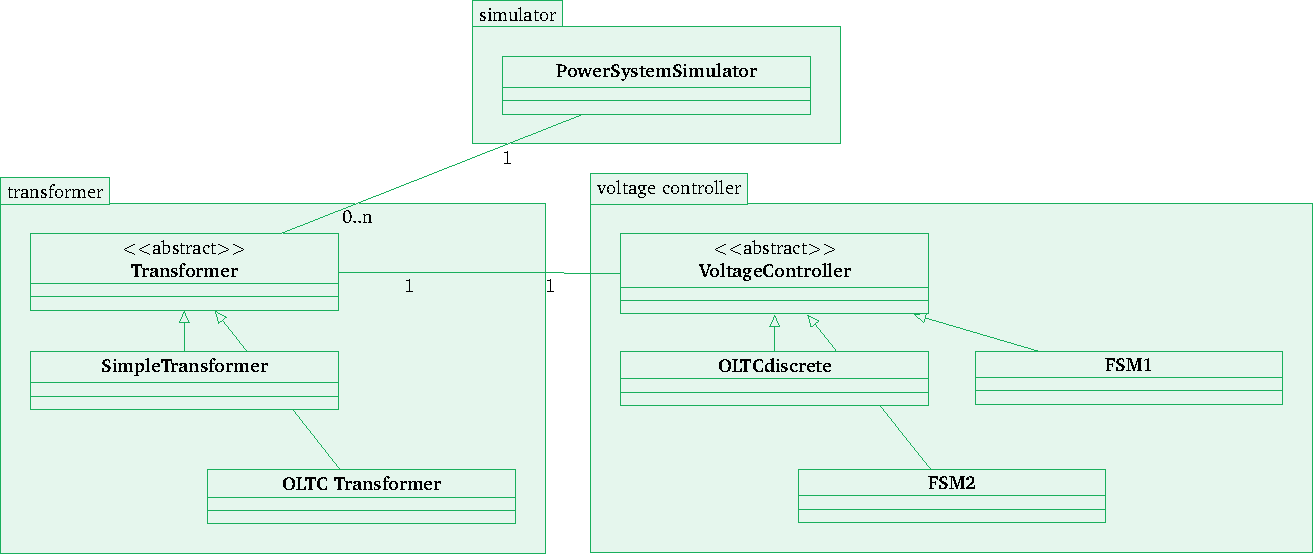
\includegraphics[angle=90, height=18cm]{./tikz_graphics/images/software_structure.pdf}%{modeling/diffpssi_trafo_architecture.png}
        \caption[Architecture of the implemented models in \textit{diffpssi}]{Architecture of the implemented models in \textit{diffpssi}; Using abstract classes for correct interfaces and improved reusability; only necessary packages, modules and classes are depicted}
        \label{fig:transformer-architecture}
\end{figure}

The main class for the Power System Simulation, hosting the central data structures and results is called \textit{PowerSystemSimulator}.
Models, busses, lines, but also transformer objects are connected to each other, and on top of that referenced in the main simulation object as groups represented by lists.
The transformers shall be connected in the same way as before, but differing from the old transformer considering just the serial impedance, a simple non-tapping transformer sall be integrated next to a longitudinal tap-changing one.
The room for possible extension, meaning phase shifters or mixtures of these models can be kept by using a abstract class as interface.
This forces the inheritating classses to override the necessary methods, have at least the mandatory attributes.
Copying existing and functional structures is easier as well.

The transformer itself is just a mathematical representation of the pi model, considering a serial impedance and two shunt branches.
Connected control units shall be excluded from this, to ensure modularity as well. 
Therefore a lot of different control tweaks can be easily implemented and tested.
To provide a consistant interface here as well, the abstract class \textit{Voltage$\_$Controller} is used.
Within this thesis implemented are a discrete and a continuous \acs{OLTC} controller, and two discrete \acs{FSM} controllers.
These reference to the standardized control blocks as well, e.g. PT1 or Integrating elements.

%%%%%%%%%%%%%%%%%%%%%%%%%%%%%%%
\subsection{Implementing a \texorpdfstring{$\Pi{}$}{}-Representative Circuit with Variable Ratio}

Before detailing in the software side of the implemetation, some mathematical differences are explained.
This results on the one hand from the major differences in the standard literature, especially between \textcite{machowski_2020} and \textcite{kundur_2022}, resp. \textcite{milano_2010}.
On the other hand, these differences occur as well in the comparative and validation simulation software \textit{DIgSILENT PowerFactory}.
The use of these different models is described in its technical reference manual \quelle. 

%%%%%%%%%%%%%%%%%%%%%%%%%%%%%%%
\subsubsection{Mathematical Description and Definitions}

\sidenote{Important definitions and literature differences}
Firstly it is important to comment on the use of indices in this thesis, and especially following for this chapter.
The index 1 is always referring to the \acs{LV} side, the index 2 to the \acs{HV} side. 
The impedances can be concentrated and related to either the \acs{LV}, or as usual to the \acs{HV} side of the transformer. 
The in \autoref{sec:trafo-model} used derivation is using a relation on the \acs{HV} side.
The same accounts for the definition of the \acs{OLTC} ratio $\underline{\vartheta}$.     
The \acs{OLTC} ratio $\underline{\vartheta}$ in this thesis is always placed on the HV side.
% If one wants to place this ratio on the \acs{LV} side, the in this thesis defined ratio has to be used reciprocal.
% For the simulation tool, this is crucial to understand and define correctly in order to acquire correct results.

\sidenote{Definition OLTC ratio}
This thesis focusses on an ideal tap changer model at first, other possible considerations from \autoref{sec:further-considerations} are neglected.
As vector groups are as well not considered, the tap ratio stays solely a rational number.
Like previously mentioned, and consequently described, the ratio $\vartheta$ is then placed on the \acs{HV} side of the transformer.
The \acs{OLTC} ratio $\vartheta$ is then defined as:
\begin{align}
        \vartheta_\mathrm{HV} &= 1 + k \cdot \Delta v \label{eq:tap-ratio-hv} \\[6pt]
        \text{with } k &\in [k_\mathrm{min};k_\mathrm{max}]; k_\mathrm{min} \equiv  -k_\mathrm{max} \label{eq:tap-pos}
\end{align}
Within this definition, $k_\mathrm{min}$ defines the minimum tap position, $k_\mathrm{max}$ the maximum \acs{OLTC} position. 
The variable $\Delta v$ defines the change of the ratio in percent for alterning one position.

% \sidenote{Representation of\\Vector Groups}
% Voltage angle shifting through the influence of vector groups, meaning a different wiring and thus magnetic coupling of the transformer can be expressed within the transformer model. 
% By mathematically applying a turning vector with the length of one to the overall tap ratio, this can be included in the model. 
% Mathematical, this is expressed by the following equation. 
% The characteristic number $n_\mathrm{T}$ is relating to to angle, with one step being equal to $30^\circ$ angle ratio.
% \begin{align}
%         \underline{a}_\mathrm{T} &= \exp(j \cdot n_\mathrm{T} \cdot \frac{\pi}{6}) \label{eq:vector-group}
% \end{align}

\subsubsection{Mathematical Different Representations}

\sidenote{Relation to the LV side}\mycomment[MK]{Rewrite this section to just Machowski style and its difference -> less confusion}
When one either wants to relate the transformer admittance, or the tap ratio to the \acs{LV} side, a different admittance matrix definition has to be used.
The admittance matrix is then defined as:
\begin{align}
        \underline{\mab{Y}}_\mathrm{\Pi,T}&= 
        \begin{bmatrix}
            \underline{Y}_\mathrm{T} & -\underline{\vartheta}\underline{Y}_\mathrm{T} \\
            \underline{\vartheta}^*\underline{Y}_\mathrm{T} & -\underline{\vartheta}^*\underline{\vartheta}\underline{Y}_\mathrm{T}
        \end{bmatrix} \label{eq:admittance-oltc}
    \end{align}
The following mathematical result leads to a necessary change in the software implementation.
Either \mycomment[MK]{Is this actually the case? Or is it a different condition?}
\begin{itemize}
        \item the admittance matrix bus indices have to be changed,
        \item the tap ratio has to be reciprocal according to \autoref{eq:tap-ratio-lv}, or
        \item using the \acs{HV} side admittance matrix, but changing the tap ratio definition and the bus indices.
\end{itemize}
These different ways of variable and placing definitions also characterize the ways, the admittance matrix of the \acs{OLTC} transformer is derived from either \textcite{machowski_2020}, versus \textcite{kundur_2022}, \textcite{milano_2010}, or \textcite{burlakin_2024}.
Another thought or way of representing a transformer with off-nominal ratio is described in the appended \autoref{app:current-injection-model}.
\begin{align}
        \vartheta_\mathrm{LV} &= \frac{1}{1 + k \cdot \Delta v} \label{eq:tap-ratio-lv}
\end{align}

\subsubsection{Design and Implementation of Algorithmics}

\sidenote{Necessary methods}
As afore described in the general architecture of the extension, interfacial methods and attributes are implemented.
Starting with the necessary methods, which can be devided into expectations from the framework itself, the operational unit type transformer, and the novel consideration as dynamic model.
From the framework itself, mainly the three methods \textit{initialize()}, \textit{enable$\_$parallel$\_$simulation()}, and \textit{get$\_$value()} are included.
All submodels have to be initialized with the preset of the measurement voltage at the to be measured bus. 
This accounts only for the \acs{OLTC} related transformers, all others pass this functionality.
To enable parallel simulations, all attributes have to be set as tensors in the expected format of the simualtions.
This is achieved trough multiplying the value with a tensor of the shape $(1, {parallel\_sims})$.
For accessing additional, or partly calculated values of interest in the model, the last method is computed.
Although this is currently also an empty function, it can be extended and called by the recorder function of the simulation framework.

Necessary methods from the transformer unit type are the calculation of the static and the dynamic admittance matrix.
As for the transformer, and the current goal of implementation, both methods are identical.
If one would want to implement also an automatic tap position configuration for load flow solving, this would provide the sufficient interface.
In the method \textit{calc$\_$admittance()}, the afore described transformer admittance matrix is calculated and inserted into the system admittance matrix at each time step.
In the begining of the \acs{OLTC} transformer, the current measurement bus voltage is aquired and handed to the output function of the connected voltage controller.
This output function is giving back the transformer ratio dependent on the current bus voltage. 
The transformer ratio is the set as an attribute and the admittance then can be calculated and updated.
As an initial value for performing load flow analysis, this ratio is set to $1$ p.u.

In order to consider this model as dynamic, three methods have to be implemented in the transformer itself: \textit{differential()}, \textit{get$\_$state$\_$vector()}, and \textit{set$\_$state$\_$vector()}.
As the transformer itself is containing no dynamics, buit its connected controllers are, these methods solely call the methods in the controllers accordingly.

\sidenote{Necessary attributes}
The necessary attributes of the transformers alowing the functions to work properly are implemented as following.
The admittance matrix is always also set as attribute.
This allows for evaluation and mapping through the recorder function.
Every transformer has a name, a resistance, a reactance and a susceptance attribute, as well as the transformer ratio $u$, resp. $u_\mathrm{l}$ for the solely longitudinal part.
For the vector group angle rotation, the attribute theta is added.
Additionally, the mandatory system related variables for the system base apparent power, the transformer apparent power, the voltages at both busses, and the parallel simulations are necessary.
Considering the direction of the transformer in the system, the set of variables declaring the bus name, id, and voltage of the \glqq from\grqq~bus is partly defining the installation.
On top of these, tap side and the measurement bus are completing the clear identification.

\sidenote{Comments on the installation}
Focussing more on the installation direction, following procedure is applied in the calculation of the admittance matrix, as it is handed over to the simulation just as tensor.
A dictionary would be possible as well, as it would possible to namely declare the tap side and non tap side index resp. impedance.
As used attributes, the attribute \textit{from$\_$bus} and \textit{tap$\_$side} receive either the flag \textit{hv} or \textit{lv}.
For the later attribute the allocation is in the responsibiliity of the user, the first one is allocated through checking the voltages of the busses.
If the \textit{from$\_$bus} is the lower value of the voltages, the value \textit{lv} is assigned, and other way round.
The admittance is then calculated for the base scenario, if the tap side of the transformer is not the from bus.
For this scenario \autoref{eq:admittance-matrix-pi} is used.
If the values match, then the admittance matrix indices are switched, and the admittance matric is set as
\begin{align}
        \underline{\mab{Y}}_\mathrm{\Pi,T}&=\underline{Y}_\mathrm{T} \cdot
        \begin{bmatrix}
                \frac{1}{\underline{\vartheta}\underline{\vartheta}^*} & -\frac{1}{\underline{\vartheta}^*} \\
                -\frac{1}{\underline{\vartheta}} & 1
        \end{bmatrix}. \notag
\end{align}

% \sidenote{Aditional considerations}
% \commenting{
%         Additionally interesting extensions:
%         \begin{itemize}[nosep]
%                 \item In which direction the matrix has to be inserted?
%                 \item Transformer types
%                 \item Measurement side detection for interface towards Tap changer control
%         \end{itemize}
% }


%%%%%%%%%%%%%%%%%%%%%%%%%%%%%%%
\subsection{Tap Changer Control Modeling}
\label{sec:modeling-tap-changer-control}

\sidenote{General interface structure}
As the tap changers, or voltage controllers for the longitudinal ratio of an \acs{OLTC}, are solely controllers, and therefore can also be dissembled in just control blocks, the necessary methods for integration in the module \textit{diffpssi} are limited.
Therefore the abstract base class, used as an interface class here, is containing the funtions \textit{differential()}, \textit{get$\_$state$\_$vector()}, \textit{set$\_$state$\_$vector()}, and \textit{get$\_$output()} for the control purposes.
Adiitionally, as every other dynamic class, both methods \textit{initialize()} and \textit{enable$\_$parallel$\_$simulation()} are included in the same way as described before as well.
In case it is needed, every controller is specifying the function \textit{update$\_$vref()}, to update the reference voltage of the control. 
The only varied standard method is \textit{get$\_$output()}, but additional needed ones are necessary dependent on the controller.
These methods are detailed in the subsequent parts of this subsection.

\sidenote{Deadband block}
Before going deeper into the control loops, two basic control blocks are implemented into the framework.
The first one is the realization of a deadband block.
This means that if the input value is smaller than a defined threshold, the output will be zero, otherwise it is returning the input value.
The differential function for this block is not necessary, as it is just reacting on the imput and not building up any dynamics or relations towards previous inputs.
The only necessary concern is the enabling of parallel simulations as well, to stay consistent with data types in the calcualtion.

\sidenote{Integrator block}
The second implementated basic block is an integrator, commonly knwon as I-block in control engineering.
This block has got relations to previous inputs and therefore a differential function, as well as methods for setting and reading the state vector.
This attribute is a storage for the state in the previous timestep, with the differential the next state can be calucated.
As the method \textit{get$\_$output()} is only called by the models, this is the connection to input variables.
An attribute input is set to the handed over value from that function, enabling the differential to be calculated.
Additionally, the output is set to the current state of the control block times a constant multiplication factor $k_\mathrm{i}$ of the integrator.
This integrator is extended by the possibility to set an limiter, as well to externally reset the state and the input variables of the object.
The differential function for an integrator is the input variable times the time step.
As this multiplication is done in the solver function of \textit{diffpssi}, the return of te differential is solely the input value.
The last part is the initialization process, where the first output of this block has to be set, meaning setting the current initial state as the wished or needed output devided through the mulatiplication factor $k_\mathrm{i}$.
This first output is then also returned.

\subsubsection{Discrete Control Loop}

\sidenote{General aspects\\and references}
This control method represents the currently most used and thus representative control scheme for \acsp{OLTC}. 
With the mechanic nature of the switching mechanism, the control loop can only access discrete ratios within time frames of around a few seconds. 
Such a discrete control loop is described by \textcite{milano_2011,milano_2010}. 
A scheme of this control loop is shown in \autoref{fig:discrete-control-loop}.
This control loop type is beneficial due to its accurate representability of current \acs{OLTC} abilities. 

\begin{figure}[htbp!]
        \centering
        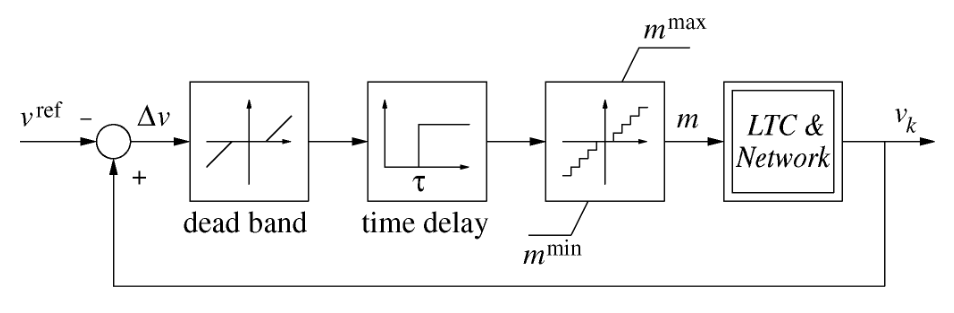
\includegraphics[width=\linewidth]{modeling/oltc_control_scheme.png}
        \caption{Discrete control loop of an \acs{OLTC}; from \textcite{milano_2011}}
        \label{fig:discrete-control-loop}
\end{figure}

\sidenote{get$\_$output()}
\commenting{
        The controller is actively changing the algebraic funtions of the simulation environment, therefore it is quasi dynamic. 
        The controller output logic is called, when updating the admittance matrix of the transformer. 
        Additionally, the differential functions of the connected simple controllers, like integrators, PT1-blocks, etc., are called by the solver and are thus part of the differential equations. 
        The logic determines the physical interpretation of the \acs{OLTC}, and therefore
        \begin{enumerate}
                \item If the OLTC has to switch,
                \item When the switching operation is finished, and
                \item What the current, or in case after a switching the new, tap ratio is.
        \end{enumerate}
        It is important to note, that this structure relies on the calculation of the dynamic admittance matrix on each time step.
}

\sidenote{switching()}
The only additional method for the discrete standard \acs{OLTC} scheme is called \textit{switching()}.


\commenting{
        \begin{itemize}[nosep]
                \item Control scheme
                \item Switching logic and behavior (voltage tracking)
                \item 
                % \item How to automatically determine switching direction?\\
                % -> switching direction dependent on what? (load-flow direction?)
                % \item Controller set points: also dependent on load flow?
                % \item How can I change the transformer control setpoints to be load flow dependent?
        \end{itemize}
}

% \lstinputlisting[caption={Output Function of the discrete OLTC controller 2},captionpos=b,style=style-python,label=lst:oltc-discrete2]{images/code/oltc-discrete.py}

% \subsubsection{Continous Control Loop}

% \commenting{Just describe the difference to the discrete \acs{OLTC}. Probably just the function get output is different, as all supplementary and attributes stay identical.}

% The implementation of an continous control scheme ia fairly straight forward.
% The desired continous block is a PT1 element with a limiter, which is already implemeted in the python module \textit{diffpssi}.
% All function say as they are descibed in the previous discrete \acs{OLTC} controller, altough the method \textit{switching()} is not needed and thus removed.
% The PT1 element is initialized with a user specified time constant, and the \acs{OLTC} tap ratio boundaries as limits.
% Additionally an error bandwith is defined for eliminating numerical noises.
% This is set to $0.01$.
% The voltage difference is then calculated, but not directly handed over to the PT1 function.
% The input to control with the PT1 is calculated by the reference voltage added to a impact factor times the voltage difference \autocite{milano_2010}.
% Typically this is three times the error, or difference.
% This cannot be realized through the gain of the PT1 block, as it would account for the complete sum.


\subsubsection{Control Schemes for the Fast Switching module}

\commenting{\textbf{ATTENTION:} Two models availabel, described in the paper, where the FSM is preferred and the 'novel' scheme where usage of FSM or OLTC ios dependent on the tap skipping and the deas band. Only the last is usable for verification!}

\commenting{
        \begin{itemize}[nosep]
                \item Describe implementation
                \item Describe benefits / drawbacks
                \item Control scheme
                \item Switching logic and behavior (voltage tracking)
        \end{itemize}

        No restrictions implemented for theta max or min! Solely limited through the max positions.
}

\sidenote{Functional basics\\of a FSM}
Describe the operational logic and structure of the \acf{FSM} first.

\sidenote{Control logic}
A control logic for a so called \acs{FSM} has been presented from \textcite{burlakin_2024}, and illustrated in \autoref{fig:fsm-control-loop}.

\sidenote{Implementation\\differences}
However, the implementation logic in Python is slightly differing from the presented scheme in \autocite{burlakin_2024}, simply for not overcomplication of the code and therefeore debugging. 
The implementation is similar to the afore discussed one of a standard \acs{OLTC} controller. 

\sidenote{Differences of variations}

\subsubsection{Characterization of the Implemented Control Schemes}
% \sidenote{Characterization\\and validation}

For characterization of the control output, two different approaches are selected.
First, a step or jump function is applied, for a maximum gradient inspection.
Further, a continous function is selected, incrementing the voltage difference on the control loop.
This could be exponential, exponential decaying, or something like linear increasing as scenario in the middle.
As the tap changer has maximum positions, and therefore also a operational band, the exponential decaying function is selected as second characterizing input.

\begin{figure}[htbp!]
        \centering
        \includegraphics[width=.7\linewidth]{development_files/validation/data/oltc_control_characterization.pdf}
        \caption[Characterization of the OLTC control loops]{Characterization of the OLTC control loop; the input function simulates the to be regulated voltage, the output functions are characterized by $o(t)=i(t) \cdot \underline{\vartheta}_\mathrm{trafo}$}
        \label{fig:oltc-control-characterization}
\end{figure}

%%%%%%%%%%%%%%%%%%%%%%%%%%%%%%%
\subsection{Experimental: Extended Ideas and Improvements}
\label{sec:experimental-modeling}

This subsection introduces a few ideas for improvements of the \acs{FSM} voltage controller.
As this is based on observations during the development, validation or analyzing case studies, one might consider going through this after understanding the thoughts of the other remaining parts.
Doing a re-read at the end would be beneficial either way.   

\subsubsection{Operational Oriented FSM Control}

\ai{
        The time constants are used in the control model to model the influnce of switching operation duration.
        This is coming from the mechanical movement of the OLTC, therefore it is the \glqq maximum possible dynamic behavior\grqq.
        The FSM doesnt't have this limitation, as it can switch after every $\sin$ period (0.02 s).
        
        Currently we can access two different operational modes: Prefer the FSM, or switching on how far is the voltage deviated in both time constants.
        This is a first, more targeted approach towards concerning dynamics in the voltage behavior, but still based on the time constants, not only limited through them.
        
        Why don't we approach a control strategy, which is only considering dynamics, and let the time constants just restrain and block the switching.
        Meaning, that the faster the voltage deviates, the more the FSM gets preferred, the slower the dynamics, the more the standard OLTC gets preferred.
        This could also lead to neglecting a dead-band, and still preventing so called tap-hunting.

        Combined with an operational oriented thought, keeping the possible switching movements of the FSM at its maximum / optimal position.
        This would mean, that in more static times, the FSM switches in its defined \glqq as neutral defined\grqq position and the OLTC is balancing the devaitions.
        One might call this a corrective supervision or monitoring.
}

\subsubsection{Alternative Tap Skipping Logic}

\ai{
        Curretnly the tap skipping logic is formulated as
        \begin{quote} \itshape
                How many times does the deadband fit into the voltage deviation?
        \end{quote}
        to determine the floored number of skips (with contraints). 
        Meaning in mathematical terms: 
        \begin{align}
                \eta(t)=\text{floor}\bigg(\frac{\vert \Delta v(t)\vert}{db_\mathrm{v} \cdot \Delta m}\bigg)
        \end{align}

        An alternative approach would be: 
        \begin{quote} \itshape
                How many switches of the FSM would the current offset voltage bring back to the reference value?
                How many times does one FSM switch fit into the voltage deviation?
        \end{quote}
        Meaning in mathematical terms:
        \begin{align}
                \eta(t)=\text{floor}\bigg(\frac{\vert \Delta v(t)\vert}{\Delta k \cdot \Delta m}\bigg)
        \end{align}
        
        Last approach should be more accurate for different pairs of preset values (deadband, added voltage per tap, etc.).
        BUT: both approaches do not consider the true effect on the dynamic loads and the grid.
        Different grid strengths could react differently on the applied transformer ratio.
}

\subsubsection{Varying the Voltage Setpoint and Target Calculation}

\commenting{
        Here, another idea of control target creation shall be mentioned. 
        Instead of a fixed bus voltage reference, the difference of both bus voltages is considered. 
        Further, the sign of that difference is used to determine the direction of the tap change.
}

\ai{
        Different things to consider here:
        \begin{itemize}
                \item \textbf{Load-flow Direction} with ranking the bus voltages in p.u. against each other,
                \item \textbf{Dynamic Setpoints} through automated calculation of target voltage (nose curves),
                \item \textbf{Different Control Input} as not with a fixed target value, but the difference between both bus voltages; thus tentiative, becuase it is not considering supporting the load, but falsly trying to prevent a wrong switching direction.
        \end{itemize}
}


%%%%%%%%%%%%%%%%%%%%%%%%%%%%%%%
%%%%%%%%%%%%%%%%%%%%%%%%%%%%%%%
\section{Application of Voltage Stability}
\label{sec:application-voltage-stability}

As previously discussed in the fundamentals of voltage stability, \autoref{sec:voltage-stability}, ensuring power quality is a secondary goal.
Concerning that voltage stability, regardless of short- or long-time evaluation, is a topic of power quality, it is hard to determine stability or instability.
In terms of static possible solutions, there are a lot of tools determing the critical points, as well as the current distance to it.
Looking into the short-term, more dynamic assessment, there are less elegant solutions. 
This thesis is trying to keep the perspective on both, short- and long term voltage stability.
The following is the approach to synthesize a toolset for voltage stability analysis, that is at least dynamically comparable.
As nose curves are a valid and popular tool, they shall be implemented first. 
Afterwards the time series calculation is tried to integrate into this static evaluation, including tap changer dependent behavior.
Lastly, a more dynamic rating of a sceario shall be computed, enabling also the confirmity with grid codes for example.

%%%%%%%%%%%%%%%%%%%%%%%%%%%%%%%
\subsection{Generation of Nose Curves}
\label{sec:nose-curves}

This section describes the implementation of a prevoiusly discussed static voltage analysis tool.
The generation of nose curves helps in finding the critical loading of the system at the bus of interest, although it is static nature. 

\subsubsection{Basic Simplification Idea}

\textcite{ajjarapu_1992, ajjarapu_2007} are presenting a method for numerical calculation of nose curves in their work. 
It is called {\itshape Continuation Power Flow} and is based on a modified Newton-Raphson method.
The differences rely in a slightly different definition of the power flow equations, considering a load factor $\lambda$.
Combined with a predictor-corrector iterative solver method, this algorithm is capable of nose curve calulation, and finding the critical loading of the system.
While in the first work \autocite{ajjarapu_1992}, only the upper part of the curve including the critical point is calculated, the second work \autocite{ajjarapu_2007} is capable of calculating the complete curve with both solutions. 
As the trade off between implementation effort and the benefits, this method is not exchanging the reduced and simplyfied one.

While this method would be appealing to implement, an additional load flow algorithm, solver, and wrapper seem not profitable for this thesis.
An idea was occuring, just iteratively using the available implemented standard Newton-Raphson algorithm, and implementing a wrapper around it.
The proposed result should be the upper and stable nose curve branch, with the critical point of active power loading.
This shall seem sufficient, as the lower branch solutions are not stable load flow solutions.

The often used parameterization of a function of voltage dependent on the active power and the power angle $\phi$ should be implemented.
In mathematical term, this is expressed as \autoref{eq:pv-mathematical}.
\begin{align}
        \vert \underline{V} \vert : P &\mapsto f(P, \phi) \label{eq:pv-mathematical} \\[6pt]
        Q : \underline{V} &\mapsto f(\underline{V}, \phi) \label{eq:vq-mathematical}
\end{align}
Under consideration of a complex representation of voltage and powers, this algorithm can calculate $V-Q$ curves as well. 
Mathematically this is expressable as \autoref{eq:vq-mathematical}.

\subsubsection{Implementation Details}

\begin{wrapfigure}[12]{r}{0.4\textwidth}
        % \vspace{-20pt}
        \centering
        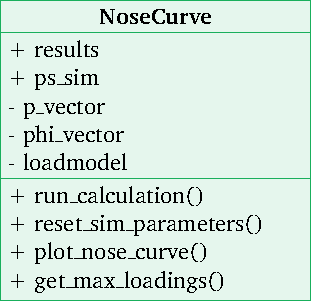
\includegraphics[width=.9\linewidth]{tikz_graphics/images/class_diagram_nosecurve_red.pdf}
        \caption{Class diagram of the NoseCurve class in the package diffpssi}
        \label{fig:nose-curve-characterization}
\end{wrapfigure}
The implementation of the nose curve generation is realized as a class in the package {\itshape diffpssi.stability$\_$lib.voltage}.
Its class diagram with all attributes and methods is shown in \autoref{fig:nose-curve-characterization}, an extended version is included in \autoref{app:nose-curve}.
For an easy and generic use of the {\itshape diffpssi} package, {\itshape PowerSystemSimulation} objects are used, as well as the function {\itshape do$\_$load$\_$flow()} from the package.

As the afore mentioned idea, the method for running the calculation is a iterative wrapper of the load flow calculation. 
This can be as well applied for mutiple busses as a list input.
At first, the grid and therefore models of the {\itshape PowerSystemSimulation} object has to be cleared with the method {\itshape reset$\_$sim$\_$parameters()}.
Then the active power vector is iterated as load input, together with the power angle $\phi$ for the reactive power in the model.
Important to note here, is the usage of an {\itshape **kwargs} argument.
The callable for the model is called with load parameters for each load bus as the Bus name, and a list with active and reactive power.
The initials of this grid callable are used as the standard values, so only one bus can be varied at a time.
The result is saved as a {\itshape pandas DataFrame} in a dict, with the keys being the bus names.

The method {\itshape plot$\_$nose$\_$curve()} is used to plot the results, and is using the {\itshape matplotlib} package.
Further, the method {\itshape get$\_$max$\_$loadings()} can provide details about the critical point.
Giving back a dict with keys as bus names, the values itself are dicts with key of the power angle parameter $\tan \phi$ and the values as {\itshape pandas DataFrame}.
The contained details are maximum active power $P_\mathrm{max}$, the reactive power $Q$ at this point, and the voltage magnitude $\vert \underline{V} \vert$ at the bus.

\sidenote{Parameter variation Nose Curves}
Additionally, the method set \textit{run$\_$variation$\_$calculation()} and its connected automated plotting method \textit{plot$\_$nose$\_$curve$\_$variation()} aims to calculate a nose curve parameter set uder variation of a system parameter variation.
This is realized through a callable function, enabling access to the desired object attribute.
Additionally a list of variation values as to be handed over, for iteration over it and saving the result to a dictionary.
This dictionary then can be plotted or accessed over the object as attribute.
The \acs{OLTC} tap dependent Nose Curves from \autoref{fig:oltc-nose-curve} are generated by this functionality

\subsubsection{Results of the Nose Curve Generation}

The following figure \autoref{fig:nose-curve-simple-grid} shows the generated nose curve for a simple grid as illustrated in \autoref{fig:single-line-voltage-stability}.
The grid is characterized at Bus 1, with a varying power angle as parameter $\tan \phi$.
The power angle $\tan \phi$ is used to vary the power factor of the load, thus representing different load characteristics, as
\begin{align}
        \tan \phi &= \frac{Q}{P}. \notag %\label{eq:tan-phi} \\[6pt]
\end{align}
Displayed are a few combinations with different load characteristics, leading to a different possible maximum acitve power transfer.
\autoref{fig:nose-curve-simple-comp} shows the comparison between the analytical calculation and the implemented solution.
The analytical calculation is carryied out with the method described in \autoref{sec:analytical-voltage-stability}.
For this specific example, the complete calculation, including the set of used parameters, is shown in \autoref{app:analytical-nose-curve}.
What seems conspicious is the missing lower part of the curve, meaning the second possible solution when solving the power flow equations.
Although this seems like a major drawback, the resulting curve contains all the necessary parts, where a stable solution can occur. \quelle
The solution is reaching exactly until the critical point of power transfer.

\begin{figure}[htbp!]
        \centering
        \includegraphics[width=\linewidth]{development_files/theoretical/plots/simple_load_B1_nose_curve.pdf}
        \caption[Examplary generated nose curve for a simple generator - load grid]{Examplary generated nose curve for a simple generator - load grid for various power angle level parameters $\tan \phi$; Applied on the grid of \autoref{fig:single-line-voltage-stability} with a characterization at Bus 1}
        \label{fig:nose-curve-simple-grid}
\end{figure}

\begin{figure}[htbp!]
        \centering
        \includegraphics[width=\linewidth]{development_files/theoretical/plots/simple_load_B1_nose_curve_w-theoretical.pdf}
        \caption[Comparison between the analytical calculation and the implemented solution]{Comparison between the analytical calculation and the implemented solution}
        \label{fig:nose-curve-simple-comp}
\end{figure}


%%%%%%%%%%%%%%%%%%%%%%%%%%%%%%%
\subsection{Combination of Static Methods with Time Domain Solutions}
\label{sec:comb-time-dimension}

Adding a \acs{TDS} to the static Nose Curve plot is fairly simple and straight forward.
The basic idea is gathering the demanded power by the load as additional recorder function, to overlap the diomensions voltage and power in the static plot.
Adiitionally using color alteration for the time dimension is keeping the evolvement information as well.
This data is then just added to the plot of Nose Curves.
The backgorund on why this could give a valuable inside, is simply looking into how close to the static solutions of the grid can the system stay under dymanic equalization and control processes.
The static solutions should theoretically the long-term solutions or states after the equalization processes.
As this dynamic solution is also conditional to the machine and machine controls for example, it could give explanations about missing capabilities from this point, as the nose curves just express the network limits.

Necessary for gathering the missing power information, the method \textit{get$\_$value()} has to be added to the static model \textit{Bus} as well.
There, specifically the apparent power $S$ is calculated through the sum of the models current injections.
With the basic relations
\begin{align}
        S&=\underline{V} \cdot \underline{I}^* \notag, \\
        P&=\mathfrak{Re} \{S\}\text{, and} \notag \\
        Q&=\mathfrak{Im} \{S\} \notag
\end{align}
one can then acces the active power as recorder attribute. 
Important to note here is, that the curret injection of a simple load cannot be calculated by default, as this model is solely adding a contribution to the admittance matrix of the system.
Therefore this model does not consider curretn injections.
As proposed work around, a load attribute \textit{i$\_$inj} is calculated in each iteration of the method \textit{get$\_$admittance()} in the static model \textit{Load} with the relation
\begin{align}
        \underline{I}_\mathrm{inj}=S_\mathrm{load}(t) \cdot \frac{S_\mathrm{n,sys}}{\underline{V}(t)^*}. \notag
\end{align}

% \commenting{
%         Idea here: Show the dynamic RMS simulation results in the quasi-staionary assessment techniques.
%         These are static solutions to the network, the electromechanic equalization processes should on a long-term watch result in these states.
%         With controls of the machines etc. one can obtain more or less a following of the static solutions until a certain point.
%         If the grid, or the machine, or its control units are stronger, a certain (heavy) level of load increase can be better and faster compensated.

%         Maybe interesting: Can the faster FSM not only increase the time until Voltage envelope is violated, but extend the transferred power as well?        
% }
        
%%%%%%%%%%%%%%%%%%%%%%%%%%%%%%%
\subsection{Using Voltage Envelopes for Criticality Evaluation}
\label{sec:comb-rating-tool}

\sidenote{Class\\ViolationIntegral}
The afore described method from \autoref{sec:stability-indices}, the \acs{TVI} is implemented as seperate class \textit{ViolationIntegral} in the package \textit{diffpssi}.
Automated simulations are not considered, as they do not add significant practicability.
Therefore, simply the results vector is just handed over.
The class diagram is displayed in \autoref{fig:class-violation-integral}.

\begin{figure}[htbp!]
        \centering
        \missingfigure{Class diagram VioolationIntegral}
        \caption[Class diagram for the class ViolationIntegral]{Class diagram for the class ViolationIntegral}
        \label{fig:class-violation-integral}
\end{figure}

As afore described, not only the mathematical describable envelopes are added, but the Machine Type II \acs{FRT} curves when connecting to the medium voltage grids from \autocite{vde-tar_2018,vde-tar_2023} are added as well.
Both envelopes are implemented as a function dependent on the time, giving back a vector in the length of the time vector and being comparable to the bus voltage solution from the power system simulation object.
Envelope parameters can be set with the function \textit{set$\_$env$\_$paramms()}, but can as well be read out through the function \textit{get$\_$env()}.
Here the same logic applies as with the envelope functions before, as a vector with the length of the time vector is given back.

\begin{figure}[htbp!]
        \centering
        \missingfigure{Class diagram CriticalTimes}
        \caption[Class diagram for the class CriticalTimes]{Class diagram for the class CriticalTimes}
        \label{fig:class-critical-times}
\end{figure}

\sidenote{Class CriticalTimes}
The class \textit{CriticalTimes} is added as well as displayed in \autoref{fig:class-critical-times}.
It is used to enable a calculation of all time steps, where the envelope(s) are violated.
The method accounts just the time stamp, where the envelope is cut from inside to outside, instead of returning all time steps outside of the envelope(s).
The envelopes can be added and results can be calculated through handing over a bus voltage result with time vector.
Results are stored as an attribute as well.
The enevelope functions are re-used from the class \textit{ViolationIntegral}

%%%%%%%%%%%%%%%%%%%%%%%%%%%%%%%
%%%%%%%%%%%%%%%%%%%%%%%%%%%%%%%
\section{Summary in Short and Simple Terms}

\commenting{
        Transformer equipment:
        \begin{itemize}[nosep]
                \item Two models -> One has to look out for which and which circumstances and definitions
                \item Phase shifting not possible -> Would be complex number instead of rational 
                \item Standardized interfaces and design
        \end{itemize}
        Voltage Rating Tool:
        \begin{itemize}[nosep]
                \item Combination of static and dynamic indices -> Evaluation of network capabilities, machine relation to that, evaluation of dynamic behavior, and assessment of the events
                \item (Static) Indexes would classify the distance / reserves of the system
                \item One number to compare for more or less stable
                \item Finding the weakest busses poossible with that -> Regarding complexer networks
        \end{itemize}
}